\pagebreak[5]
\subsection{The CML Metamodel (Abstract Syntax)}\label{subsec:metamodel}

The EMOF \cite{mof} model presented by figure \ref{fig:metamodel} is a simplified version of the CML metamodel:

\begin{figure}
\centering
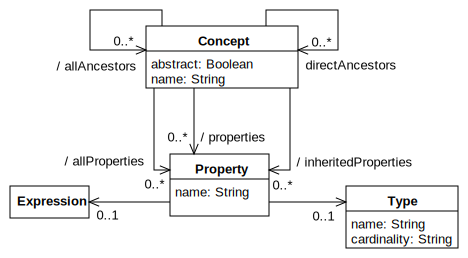
\includegraphics[width=0.8\textwidth]{language/diagram-metamodel}
\caption{This class diagram renders the EMOF \cite{mof} model defining the CML metamodel.}
\label{fig:metamodel}
\end{figure}


In the article \emph{UML and OCL in Conceptual Modeling}, 
Gogolla \cite{gogolla} shows, by mapping the UML \cite{uml} metamodel to the ER \cite{er} metamodel,
how UML models (augmented by OCL \cite{ocl} constraints) can be used to specify conceptual models.
Also, Wazlawick \cite{wazlawick} in his book systematically prescribes a method for conceptual modeling using UML and OCL. 
Since one key CML goal is enabling the specification of conceptual models
(such as those specified by ER models and UML/OCL models),
in order to present the key elements of the CML metamodel in the following subsections,
a similar approach to Gogolla's will be used (mapping the CML metamodel to the UML/OCL metamodel).

[Describe the relationships between the concepts in the diagram]

[Subsection for each key concept in the CML metamodel.]